\RequirePackage{filecontents}

\begin{filecontents*}[overwrite]{\jobname.xmpdata}
    \Title{Software Architektur}
    \Author{Projektteam 6}
    \Language{%
        de-DE
    }
    \Keywords{%
        AMOS\sep
        WS 2021/2022\sep
        Explainable Similarity Detector\sep
        Projektteam 6\sep
        Software Architektur\sep
        Laufzeit Komponenten\sep
        Code Komponenten\sep
        Zugrunde liegender Technologie-Stack
    }
    \Subject{Software Architektur}
    % \Date{2021-11-06}
\end{filecontents*}

\documentclass[%
    a4paper
]{scrartcl}

\usepackage{colorprofiles}
\usepackage[%
    dvipsnames,
    table,
    rgb
]{xcolor}

% PDF-A
\usepackage[%
    a-3u,  
    mathxmp    % mathematical letters
]{pdfx}

\usepackage[utf8]{luainputenc}

\usepackage{fontspec}
\setmainfont{Arial}

\usepackage[%
    a4paper,
    % showframe=true
]{geometry}

\usepackage{graphicx}

\usepackage[%
    automark,
    headsepline
]{scrlayer-scrpage}

% Commands
\newcommand{\leadingzero}[1]{\ifnum #1<10 0\the#1\else\the#1\fi}
\newcommand{\todayGer}{\leadingzero{\day}.\leadingzero{\month}.\the\year} 

\begin{document}

% !TEX root = ./architecture.tex

% Don't use header and footer on titlepage
\clearmainofpairofpagestyles

% Disable headlinesep 
\KOMAoption{headsepline}{false}

\begin{center}
    \vspace*{2cm}
    \Huge{Explainable Similarity Detector}\\

    \vspace*{0.3cm}
    \huge{AMOS WS 2021/2022}

    \vspace*{1.5cm}
    \large{Projektteam 6}

    \vspace*{0.5cm}
    \normalfont{\todayGer}
\end{center}

\vspace*{\fill}

\renewcommand{\contentsname}{Inhaltsverzeichnis}
\tableofcontents

\vspace*{0.5cm}

\renewcommand{\listfigurename}{Abbildungsverzeichnis}
\listoffigures

\vspace*{\fill}

\newpage

\KOMAoption{headsepline}{true}

\chead[]{Explainable Similarity Detector}

\ifoot{AMOS WS 2021/2022 - Pr. 6}
\cfoot[]{\pagemark}
\ofoot{\todayGer}

\section{Laufzeit Komponenten}

% An overview diagram of runtime components (one page)

Überblick über die Laufzeit Komponenten

\vspace*{\fill}

\begin{figure}[ht]
    \centering
    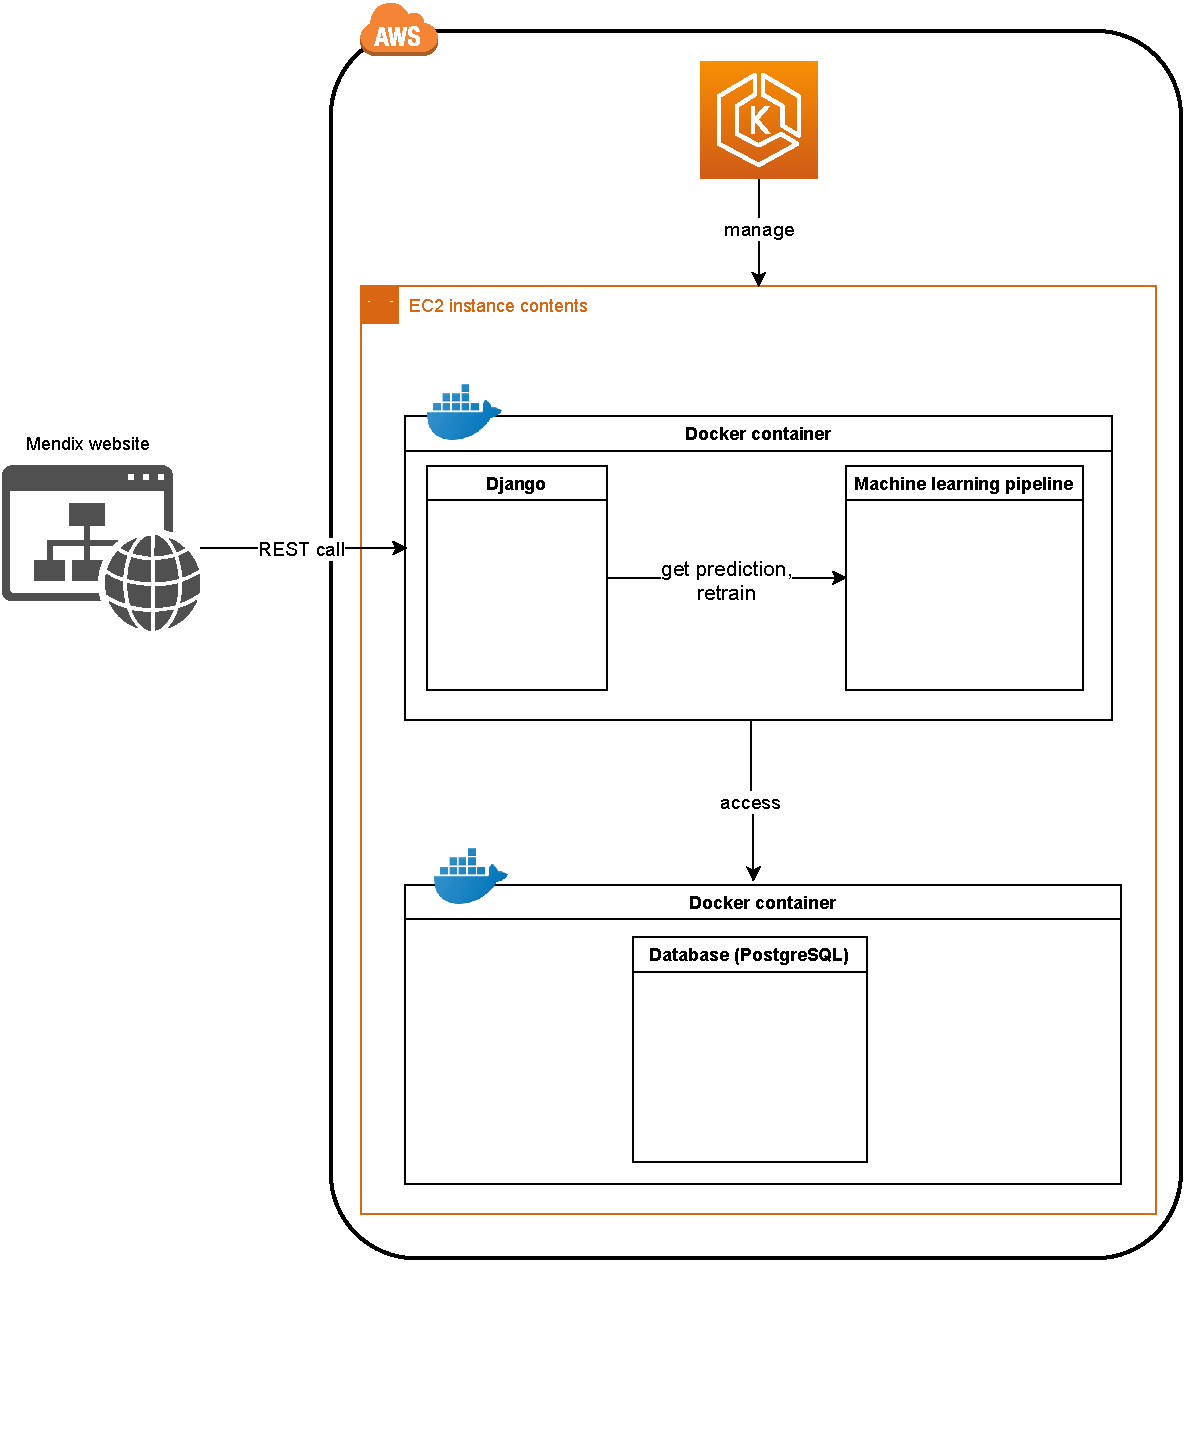
\includegraphics[%
        width=0.96\textwidth,
        clip, 
        trim=0cm 2.7cm 0cm 0cm % trim=left botm right top
    ]{../runtime-components/runtime-components}
    \caption{Laufzeit Komponenten}
    \label{fig:runtime-components}
\end{figure}

\vspace*{\fill}

\newpage

\section{Code Komponenten}

% An overview diagram of code components (one page)

Überblick über die Code Komponenten

\vspace*{\fill}

\begin{figure}[ht]
    \centering
    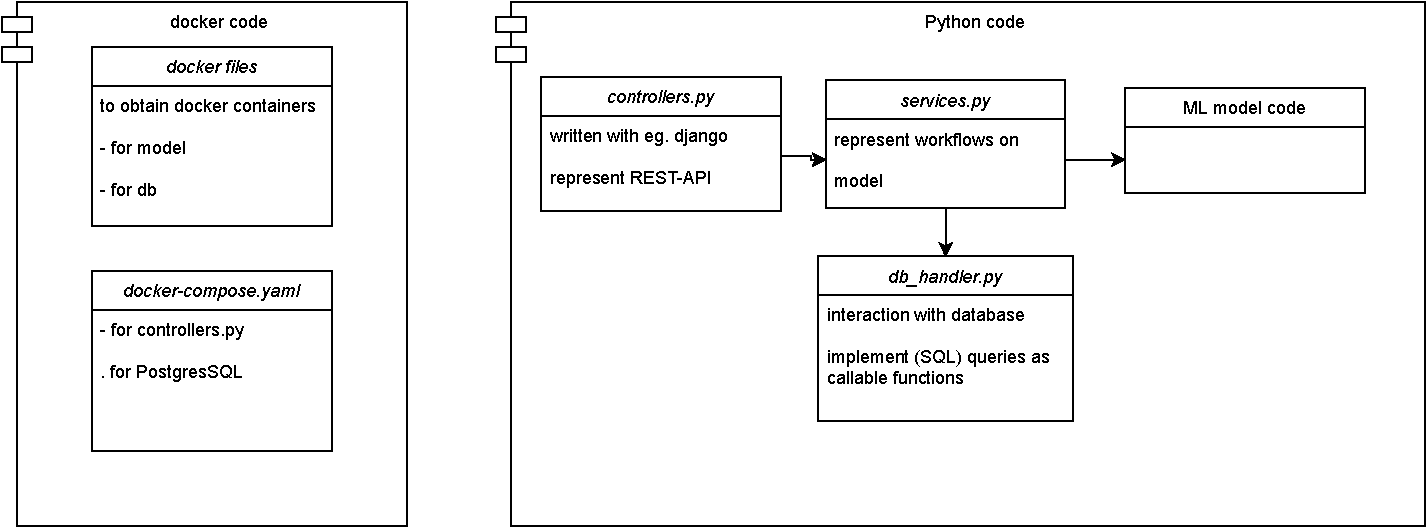
\includegraphics[%
        width=0.96\textwidth,
        clip, 
    ]{../code-components/code-components}
    \caption{Code Komponenten}
    \label{fig:code-components}
\end{figure}

\vspace*{\fill}

\newpage

\section{Technologie-Stack}

% A summary of the underlying technology stack (one page)

Zusammenfassung des zugrunde liegenden Technologie-Stacks

\newpage

\section{Textuelle Erklärung}

% A textual explanation of the diagrams and choices (one page)

Textuelle Erläuterung der Diagramme und Auswahlmöglichkeiten



\end{document}
